\chapter{New Hoeffding Tree Based Ensemble Approach}
\label{chp:algo}
In the previous chapters, we have presented the motivations, fundamental concepts for this thesis. Now, in this chapter, we present our algorithms, Size Restricted Hoeffding Tree (SRHT) and Carry-over bagging. Size restricted Hoeffding tree is extended from original Hoeffding tree algorithm and incorporates ADWIN method. Carry-over bagging is developed over the concepts of Oza online bagging approach. 
Before, discussing the algorithms, we define our problem mathematically. 

\section{Problem Statement}
Various modern application areas produce huge amount of data or so-called data streams. Most state-of-the-art stream mining methods generalize all application areas by similar streams. Assumptions are made that streams are generated from constant generators with concepts following some distribution. The concepts themselves may drift or evolve, but overall nature of the generators remain the same.

Close examination of certain application domains such as social media, WWW, telecommunication, etc. suggest that streams are decomposable in smaller sub-streams, possibly in a mutually exclusive manner. These sub-streams  can differ significantly in the way they generate or contribute to the overall stream. Some of these sub-streams are very short-lived but produce extremely high number of instances, whereas some are always present and consistently produce data but with relatively very slow speed.

Generalizing such streams with a generator that does not produce these scenarios might not properly represent these applications. Performance measures such as overall accuracy, may fail to indicate limitations of learners in such environment.

In Chapter~\ref{chp:dataset}, we demonstrate how to synthesize a data set with speed varying properties. With this type of data sets, current state-of-the-art methods face trouble in learning the slower streams. As it takes longer time to accumulate sufficient information for the concepts with slower speed, only those classifiers with larger capacity and longer lifetime would contain decision rules for slower concepts. Then again, we have usual challenges of concept drift, size of the classifier, over-fitting, etc.

With these motivations, we define our problem statement as follows:

\begin{quotation}
    \textbf{Online classification of data streams, which are decomposable into speed-varied sub-streams, with Hoeffding tree based approaches.}
\end{quotation}

\noindent Formally, given a stream $S$ of very high volume, possibly infinite, having a set of $m$ nominal or continuous attributes $X$, where each instance has a class label from a set $Y = \{y_1, y_2, \dots, y_k\}$; we want to build a classifier that is able to predict the classes of incoming instances at any given time. Note that, this definition is very general, and can be used for any of the current learners. The uniqueness lies the in nature of stream $S$. We want to improve the performance when $S$ is a composite stream of a set of sub-streams with huge contribution differences.


\section{Solution Overview}
Like all other stream learning algorithms, there are 3 most important aspects that need  to be addressed in our potential learning algorithm. These are (i) the model has to be updated to be able to classify most recent data, (ii) the model has to detect concept drifts and to be updated accordingly, and (iii) model must no grow to be very complex causing over-fitting. Along with these requirements for our problem, additionally, (iv) it needs to perform equally good for different concepts within the classes. As the arguments were made before, fulfilling this new requirement is challenging because of first two requirements. To keep the model up-to-date with the data and the concept, effect of older concepts and data need to be removed from the model. In doing so, very easily we end up losing information of the slower sub-streams. As the faster sub-streams produce high volume of data, the model is always dominated by those concepts. Slower sub-streams initially get classified wrongly, then over time when the model gathers enough information about these slower streams or concepts, new rules emerge for those concepts. However, these rules become `old'  soon with the incoming volume of faster concepts. As a result, in most of the current state-of-the-art stream mining methods, these rules will get pruned after a while to keep the model update to data and concepts.

To achieve the fourth goal, we modify few of the existing methods and use them in a combination. From the methods discussed in Chapter~\ref{chp:background}, we learned approaches of learning a decision a tree and keep it updated to the newer concepts. Based on that let's first analyze what are the possible approaches that can be taken to keep a model updated to the newer concepts and data, and how to get rid of the effect of older concepts.

\subsection{Incrementally Growing Tree}
Using methods such as Hoeffding Tree (Section~\ref{sec:bg:vfdt}) would result in an incremental tree with time. Hoeffding tree keeps itself updated by spanning the entire feature space and updating the weights values within the leaves. Theoretically, with sufficiently large learning time and diverse data instances, Hoeffding will span the entire feature space with all possible combinations.

\begin{figure}[htbp]
    \begin{center}
        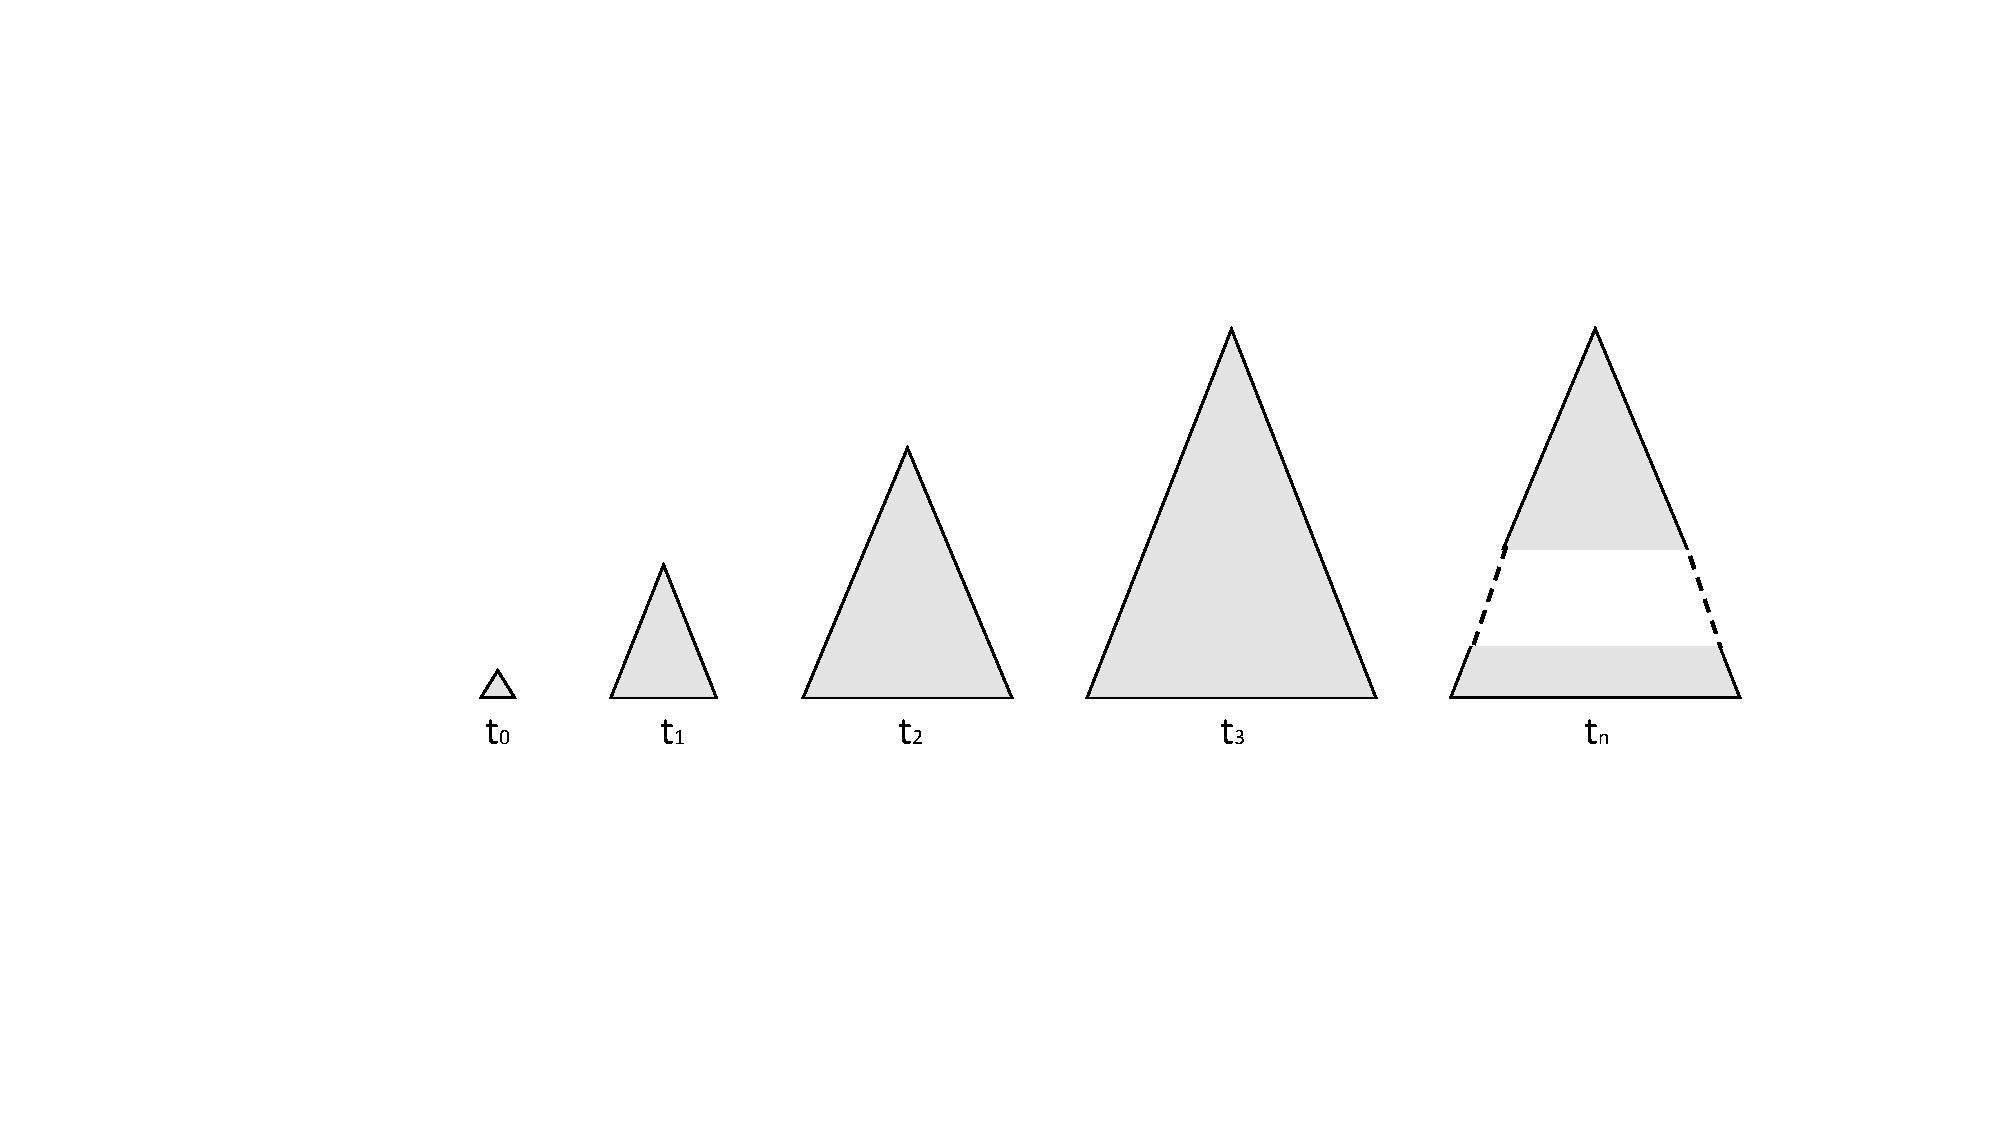
\includegraphics[width=14.0cm]{figs/infgrow.pdf}
        \caption{Incrementally expanding tree}
        \label{fig:algo:infgrow}
    \end{center}
\end{figure}

Figure~\ref{fig:algo:infgrow} shows how the size of the tree may change over time. At $t_0$, it starts with a single node, and keeps expanding as the time passes. A hypothetical corresponding decision boundaries in 2D space are shown in~\ref{fig:algo:infgrowdb}. As the figure shows, the model become complex and prone to the slightest changes in data.

\begin{figure}[htbp]
    \begin{center}
        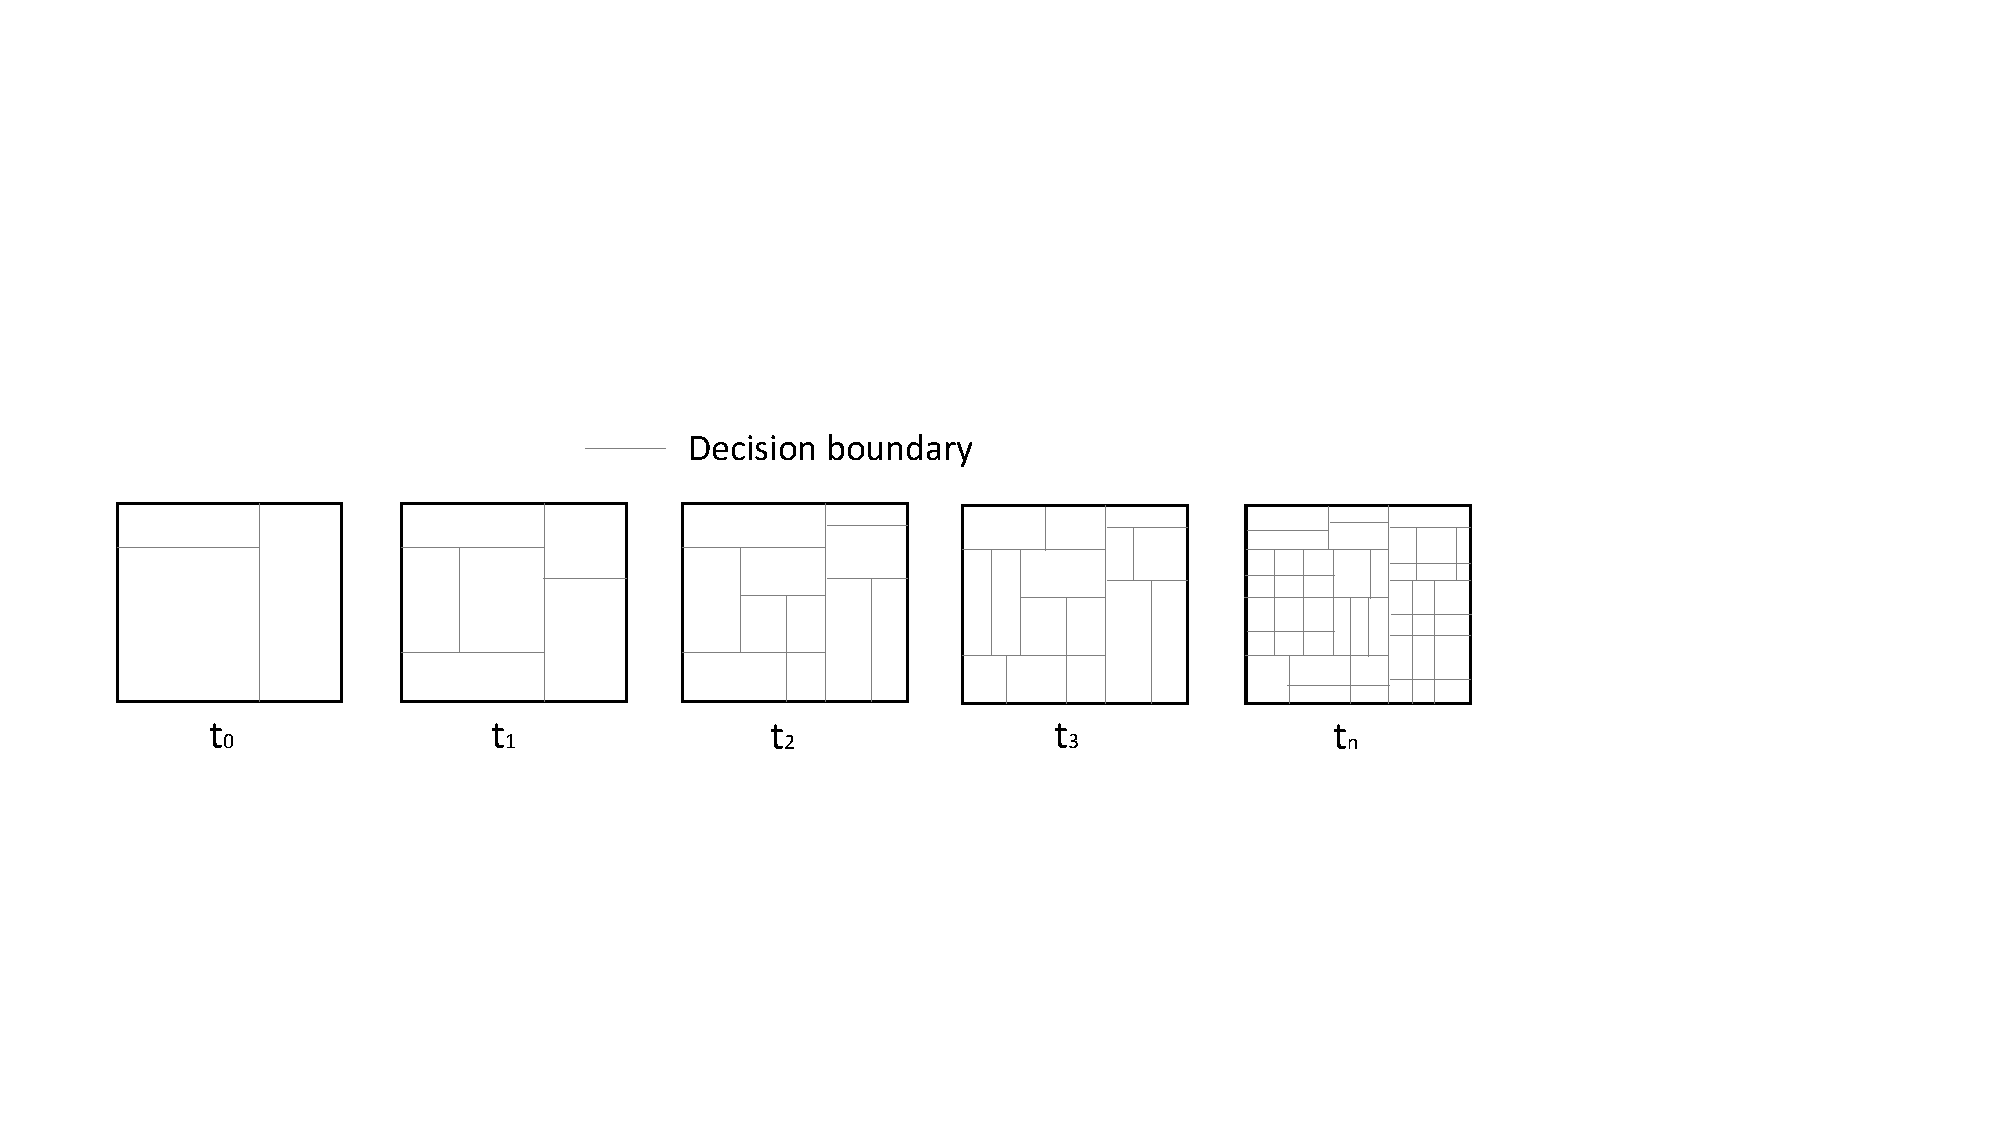
\includegraphics[width=14.0cm]{figs/infgrowdb.pdf}
        \caption{Decision boundaries for infinitely expanding tree}
        \label{fig:algo:infgrowdb}
    \end{center}
\end{figure}


\subsection{Resetting Tree}
The scheme of incrementally growing Hoeffding tree is simple and easy to implement. However, one of the major shortcomings of this approach is that, it leads to over-fitting. As there are abundance of training instances, after a period, the model starts following the instances rather than trying to realize the underlying relations. One way to stop that from happening is to reset the tree once in a while (Figure~\ref{fig:algo:reset}). This reset could be triggered by some time dependent event, or it could also be dependent on some properties of the tree. For example, depth of the tree, size or number of nodes in the tree, number of decision nodes in the tree, etc. can be used as a trigger with a maximum threshold bound.

\begin{figure}[htbp]
    \begin{center}
        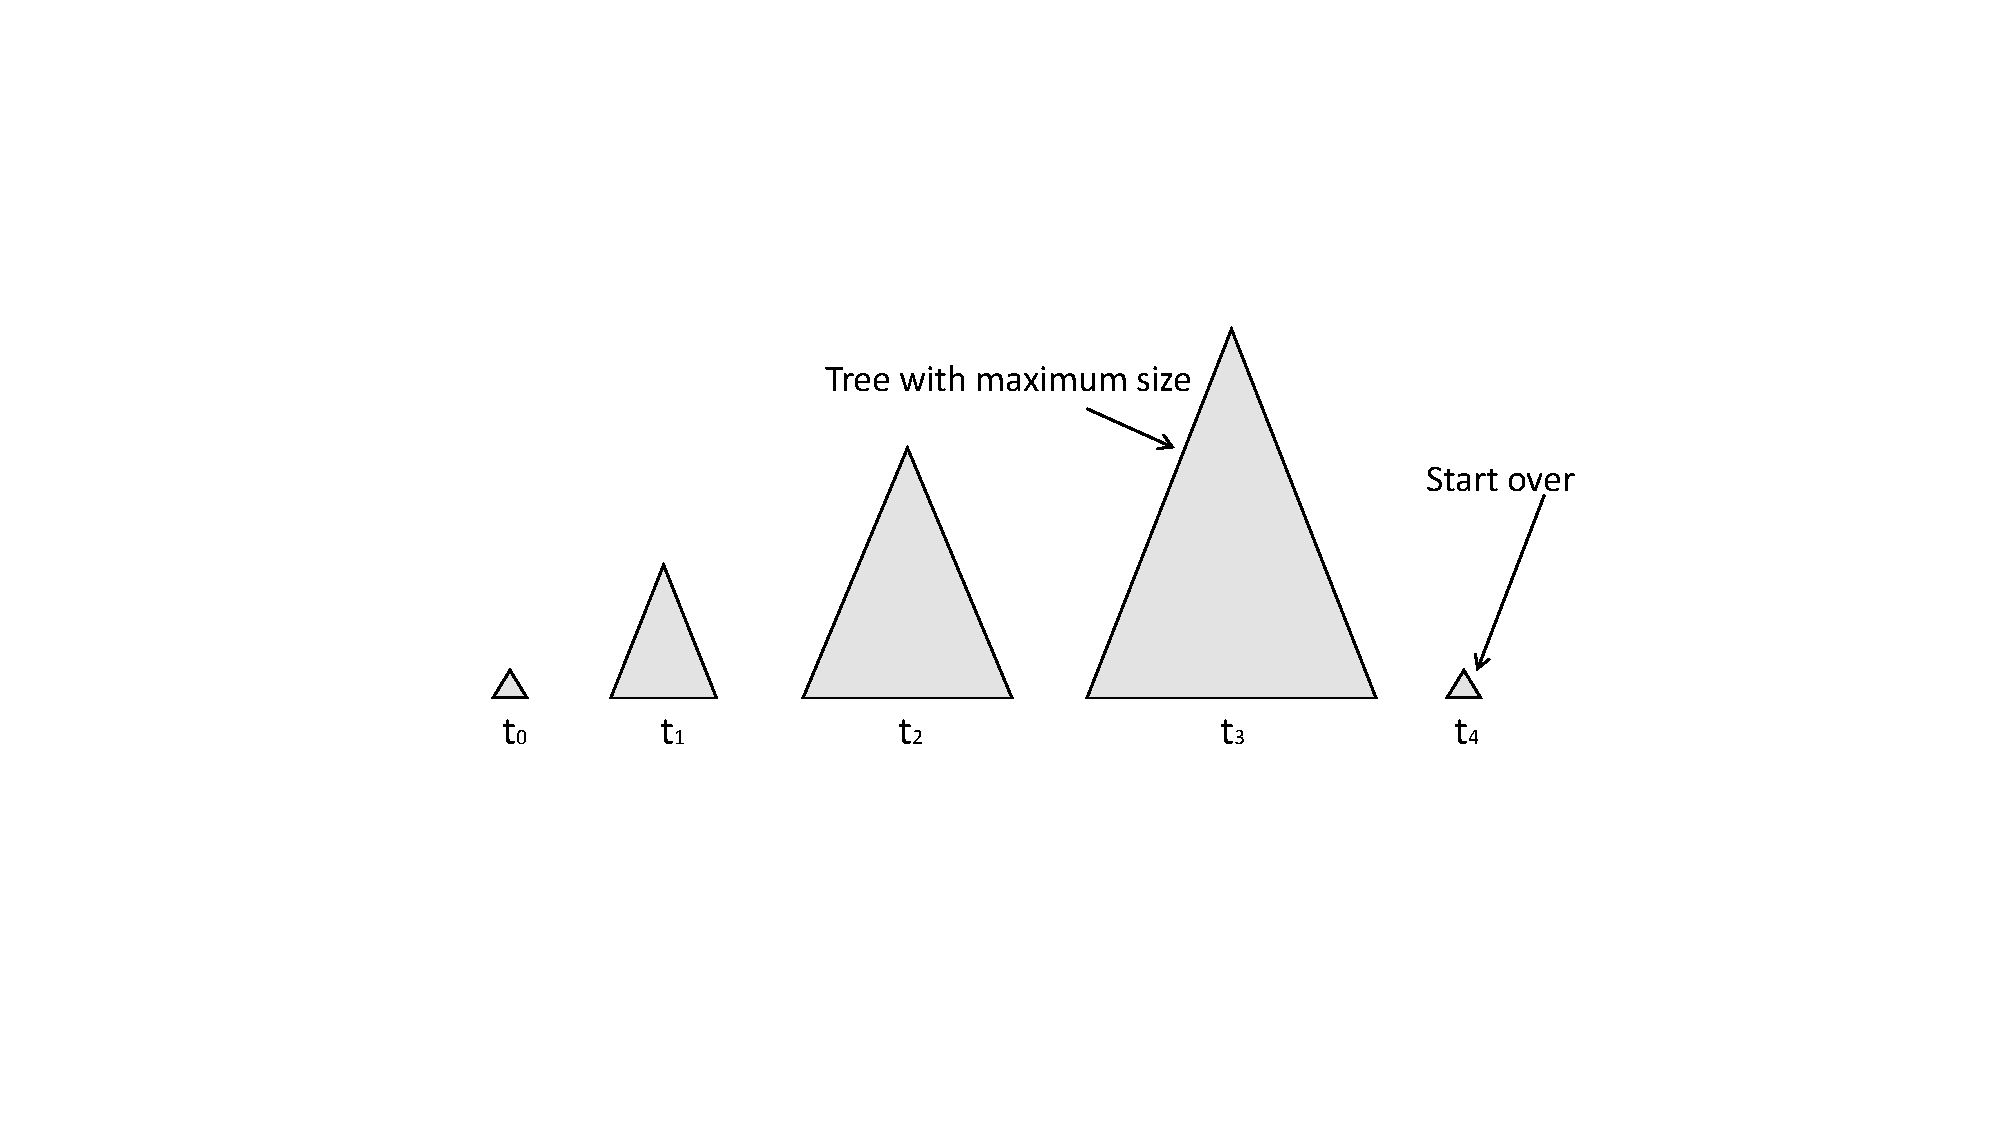
\includegraphics[width=12.0cm]{figs/reset.pdf}
        \caption{Resetting entire tree upon reaching threshold size}
        \label{fig:algo:reset}
    \end{center}
\end{figure}


Essentially, by resetting the entire tree, the model starts learning from scratch again. Every decision rule learned from observed data are lost (Figure~\ref{fig:algo:resetdb}). However, it does also get rid of all the biases for the incoming data that were present because of the observed data. In Adaptive Size Hoeffding Tree (ASHT) bagging, this reset idea has been used in association with an ensemble of different sized ASHTs (Section~\ref{sec:bg:asht}). As the size threshold is different for the trees in the ensemble, the probability of all trees being reset at once is very less. Thus, by  resetting a tree  in an ensemble allows the model to retain important information upon a reset of a tree in the ensemble through other trees. However, it is important to understand that reset of smaller trees in ensemble have lesser effect than the reset of larger trees. Smaller trees in the ensemble target recent data, and there are abundance of that. On the other hand, larger trees contain information learned over a longer period, thus also containing small but important concepts. This is exactly what we want to retain.

\begin{figure}[htbp]
    \begin{center}
        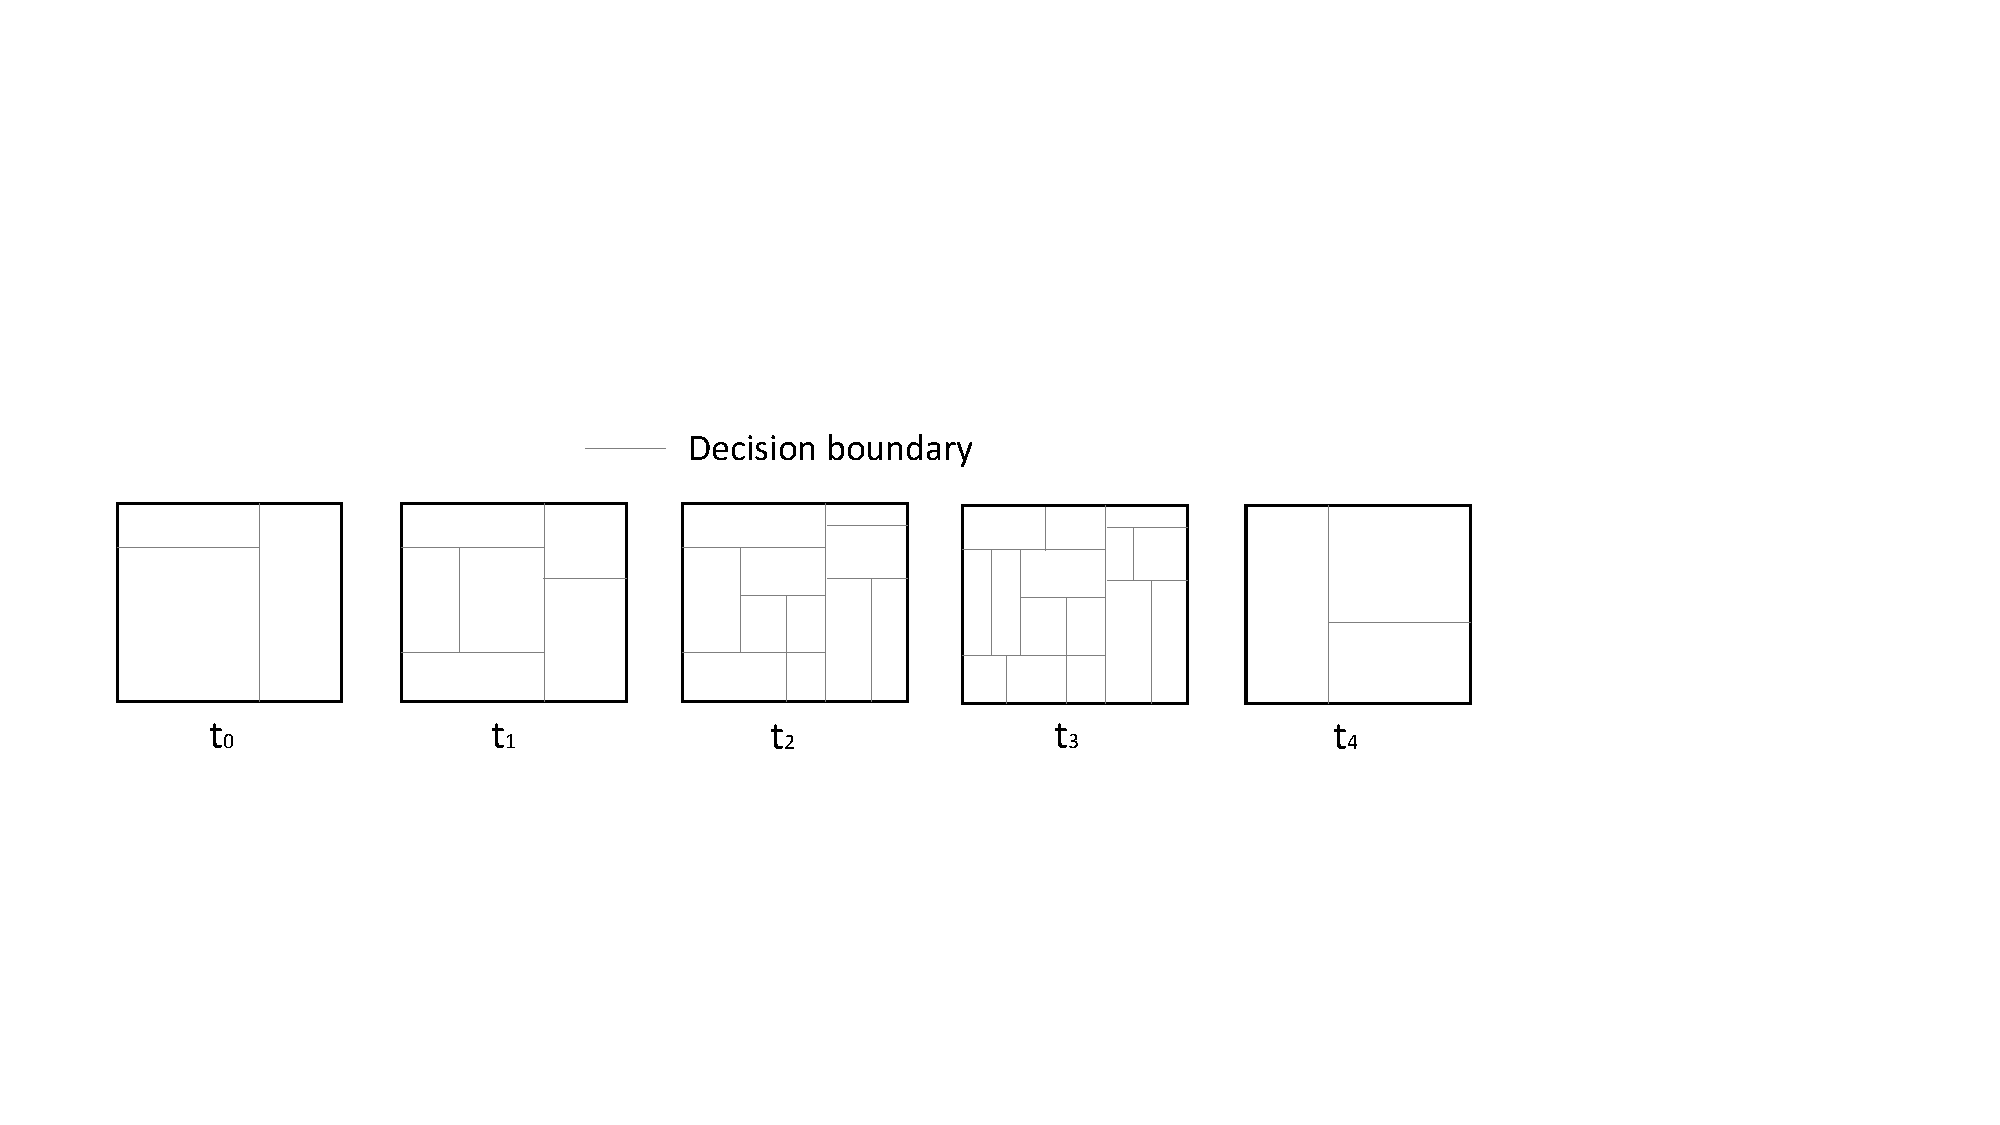
\includegraphics[width=14.0cm]{figs/resetdb.pdf}
        \caption{Decision boundaries after tree reset}
        \label{fig:algo:resetdb}
    \end{center}
\end{figure}

\subsection{Pruning by Deleting Older Nodes}
An alternate choice to resetting entire tree is to delete the older decision nodes, e.g. root or top levels. As in the Hoeffding tree, split attribute choice for each level depends on newer data from the previous level, the top level decision nodes are chosen based on oldest data segments (Figure~\ref{fig:algo:delroot}). Thus, removing the root and all its children except for the one chosen as the next root would remove the effect of the oldest data. It also allows the tree to grow again, if there is any size restriction, as the threshold (number of decision nodes) is effectively decreased by at least 1.

\begin{figure}[htbp]
    \begin{center}
        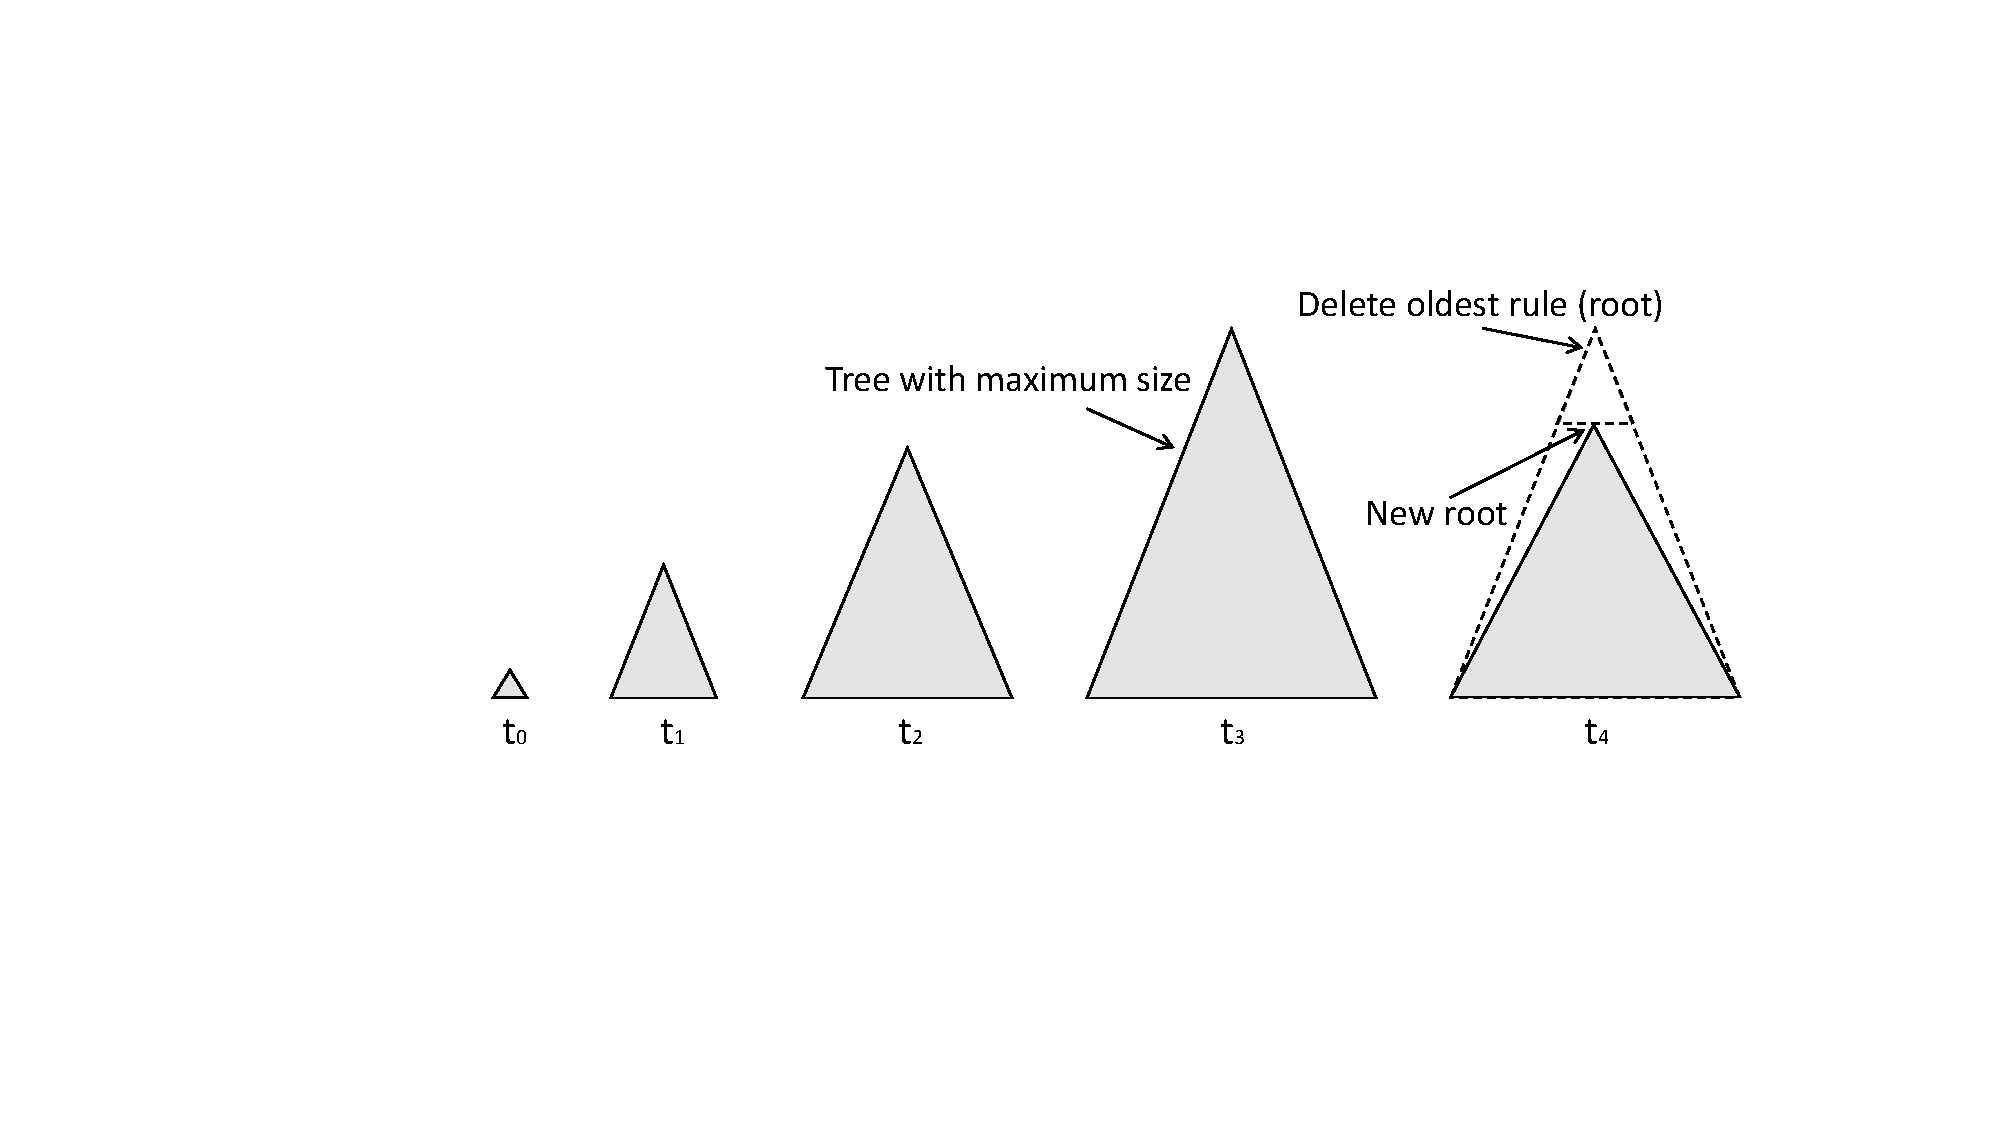
\includegraphics[width=14.0cm]{figs/deleteroot.pdf}
        \caption{Deleting the oldest branch (root) and selecting new root from its children}
        \label{fig:algo:delroot}
    \end{center}
\end{figure}

Figure~\ref{fig:algo:delrootdb} shows the changes in the decision boundary upon deleting the root. As it shows, only the earliest boundaries are deleted in this process. If the model has already become too complex, then this does not improve the situation much. But for less complex models, this should create chance for the tree to learn information within the newly merged regions. Moreover, because the order in which the checks are performed changes, the existing decision rules might change (decision class).

\begin{figure}[htbp]
    \begin{center}
        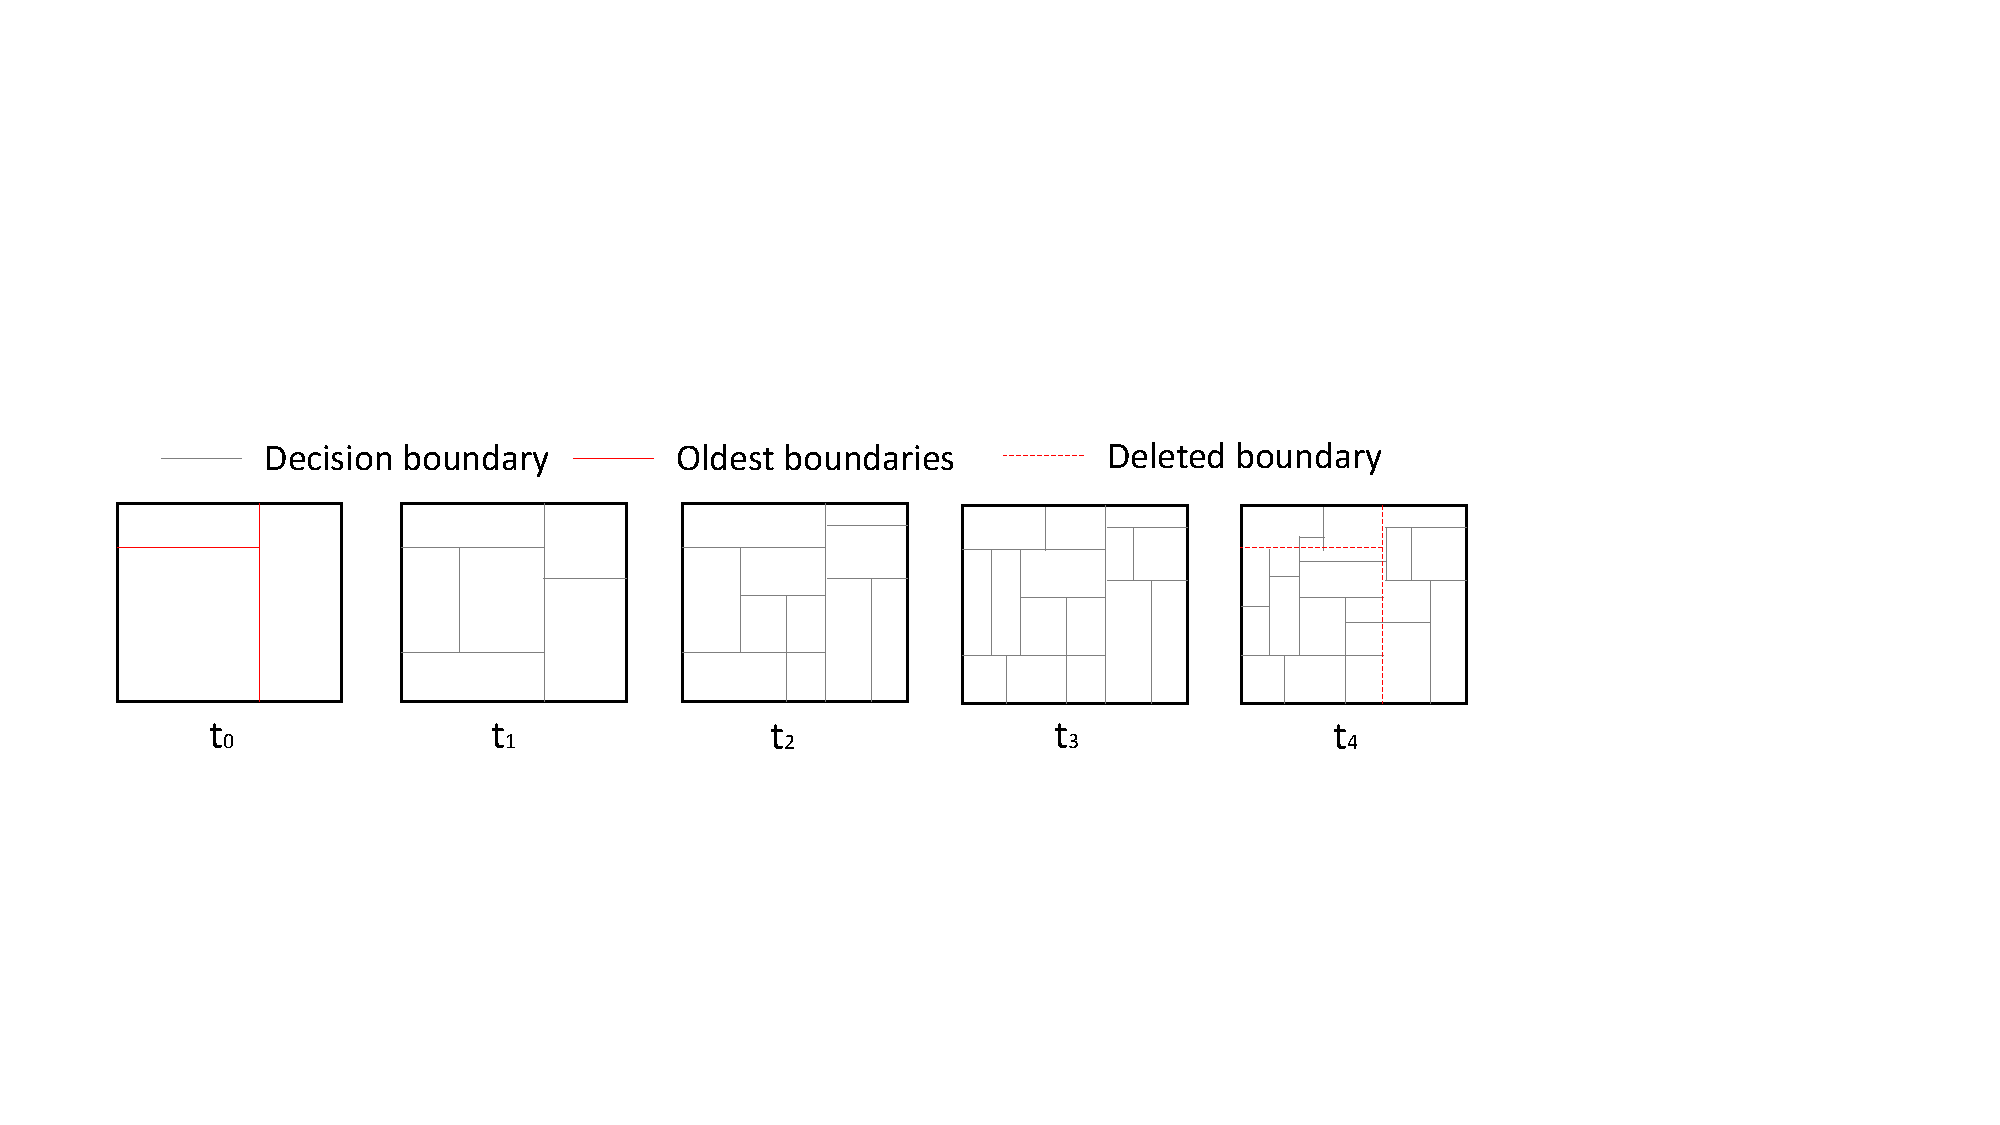
\includegraphics[width=14.0cm]{figs/deleterootdb.pdf}
        \caption{Decision boundaries after deleting root}
        \label{fig:algo:delrootdb}
    \end{center}
\end{figure}


\subsection{Pruning by Maintaining Alternate Trees}
In a different approach than deleting root or entire tree, maintaining alternate sub-tree wherever necessary can effectively maintain the model's relevance to the recent data. Adaptive Hoeffding Tree uses such approach by maintaining ADWIN (Section~\ref{sec:bg:changedetection}) to check error margin at each decision node. In case of an increase in error margin at any node, an alternate branch is initiated and learned. In the future, if there is enough evidence that an alternate branch performs better than the current one, then current sub-tree is replaced with the alternate sub-tree. Otherwise, the alternate sub-tree is deleted. Every time error margin exceeds main tree and the alternate tree, a new alternate branch is created. Thus, one decision node might have multiple alternate sub-tree. Note that, an alternate branch might get started at the root itself, and if it performs better, would change the entire tree with something new.

\begin{figure}[htbp]
    \begin{center}
        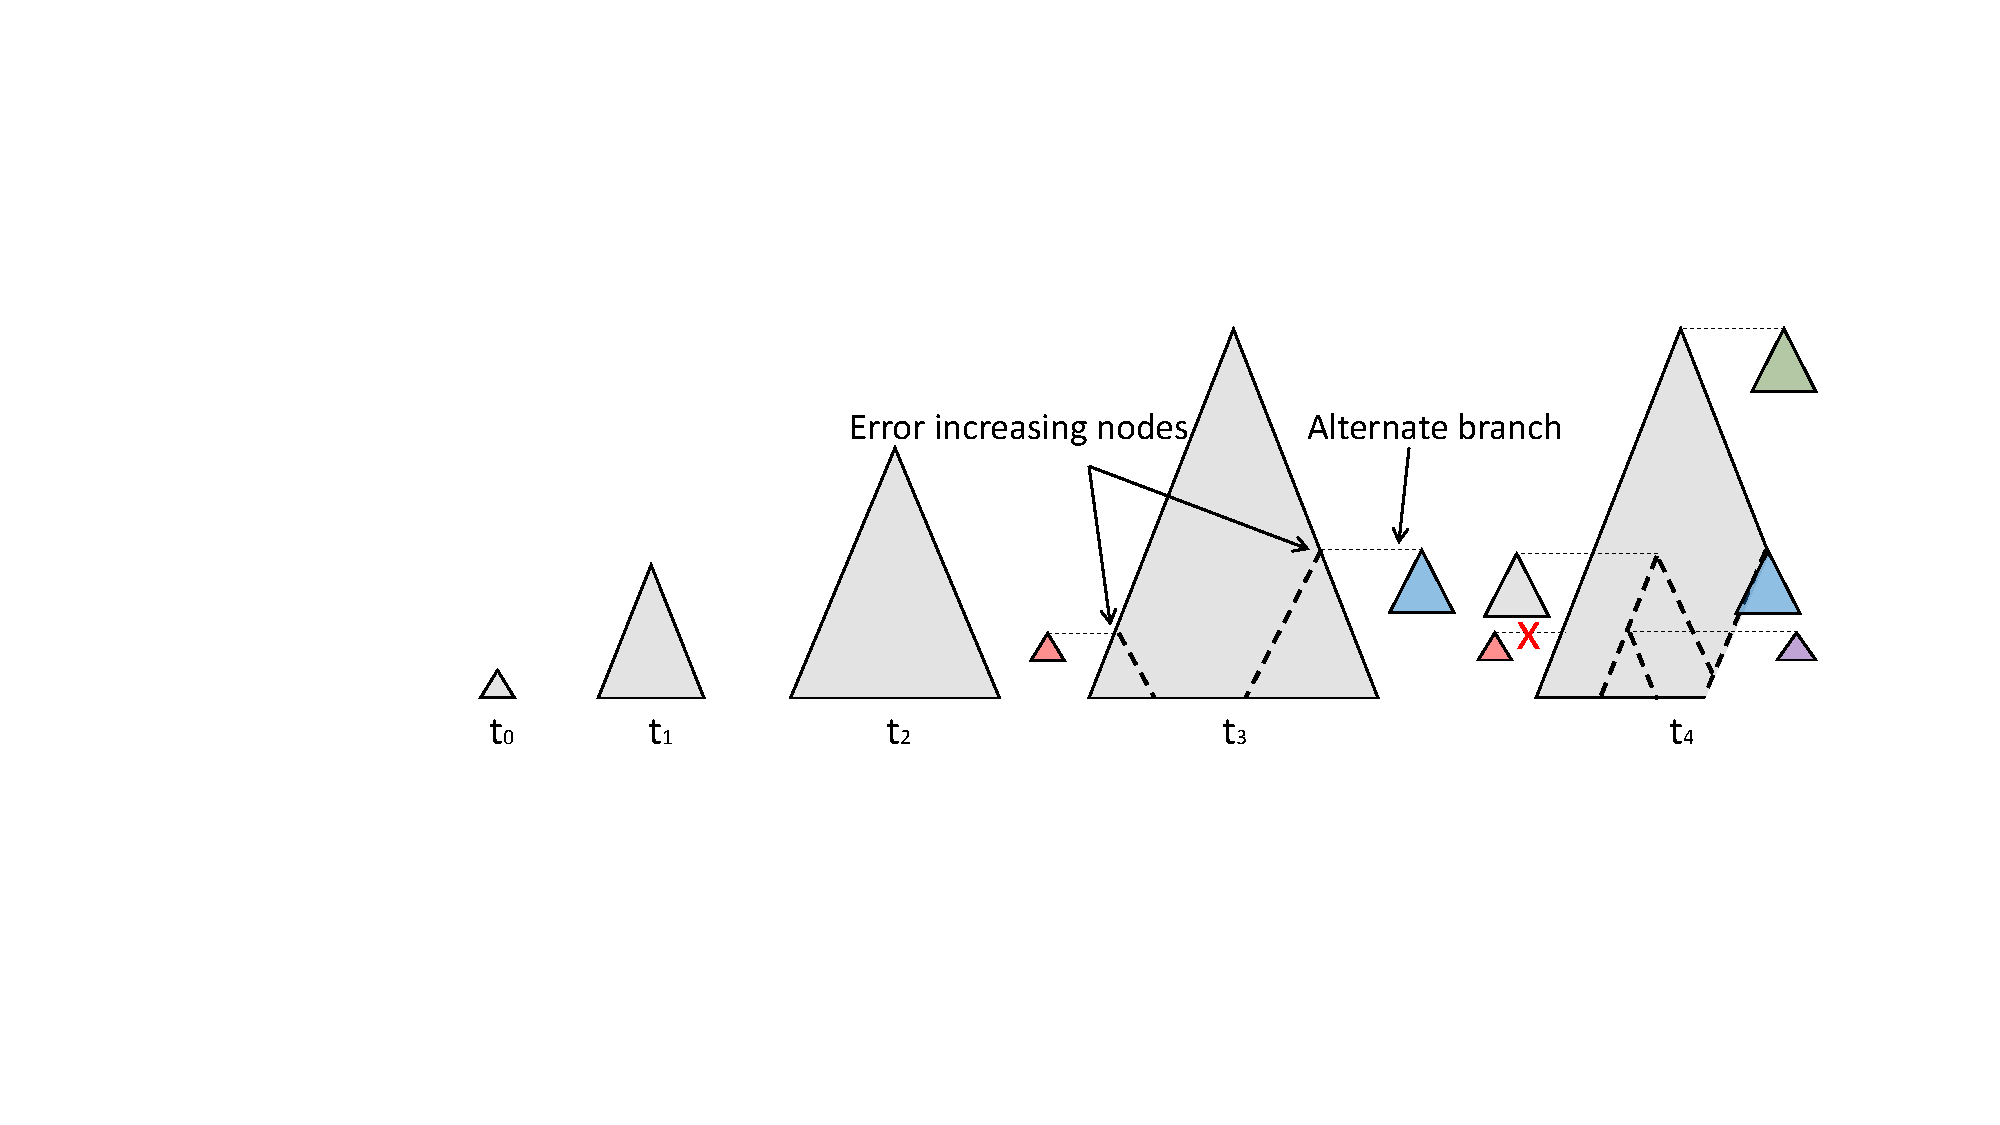
\includegraphics[width=14.0cm]{figs/prune.pdf}
        \caption{Maintaining alternate branches for pruning}
        \label{fig:algo:prune}
    \end{center}
\end{figure}

Pruning using alternate trees can effectively detect changes in the concepts. As it employs ADWIN, nodes are not immediately replaced if they start performing worse than before. Rather, it waits to confirm that an actual change in the data concepts has occurred. Otherwise, it deletes the alternate tree. This way, the model is saved from being prone to outliers and very small blocks of data from other concepts. In Figure~\ref{fig:algo:prunedb}, we illustrated how the decision could change in terms of the trees shown in Figure~\ref{fig:algo:prune}. Generally, it is expected that a block of decision boundaries will be replaced by another block. It does not necessarily need be a simpler one. Alternate trees, theoretically, can be more complex than the block it would replace in the original tree.

\begin{figure}[htbp]
    \begin{center}
        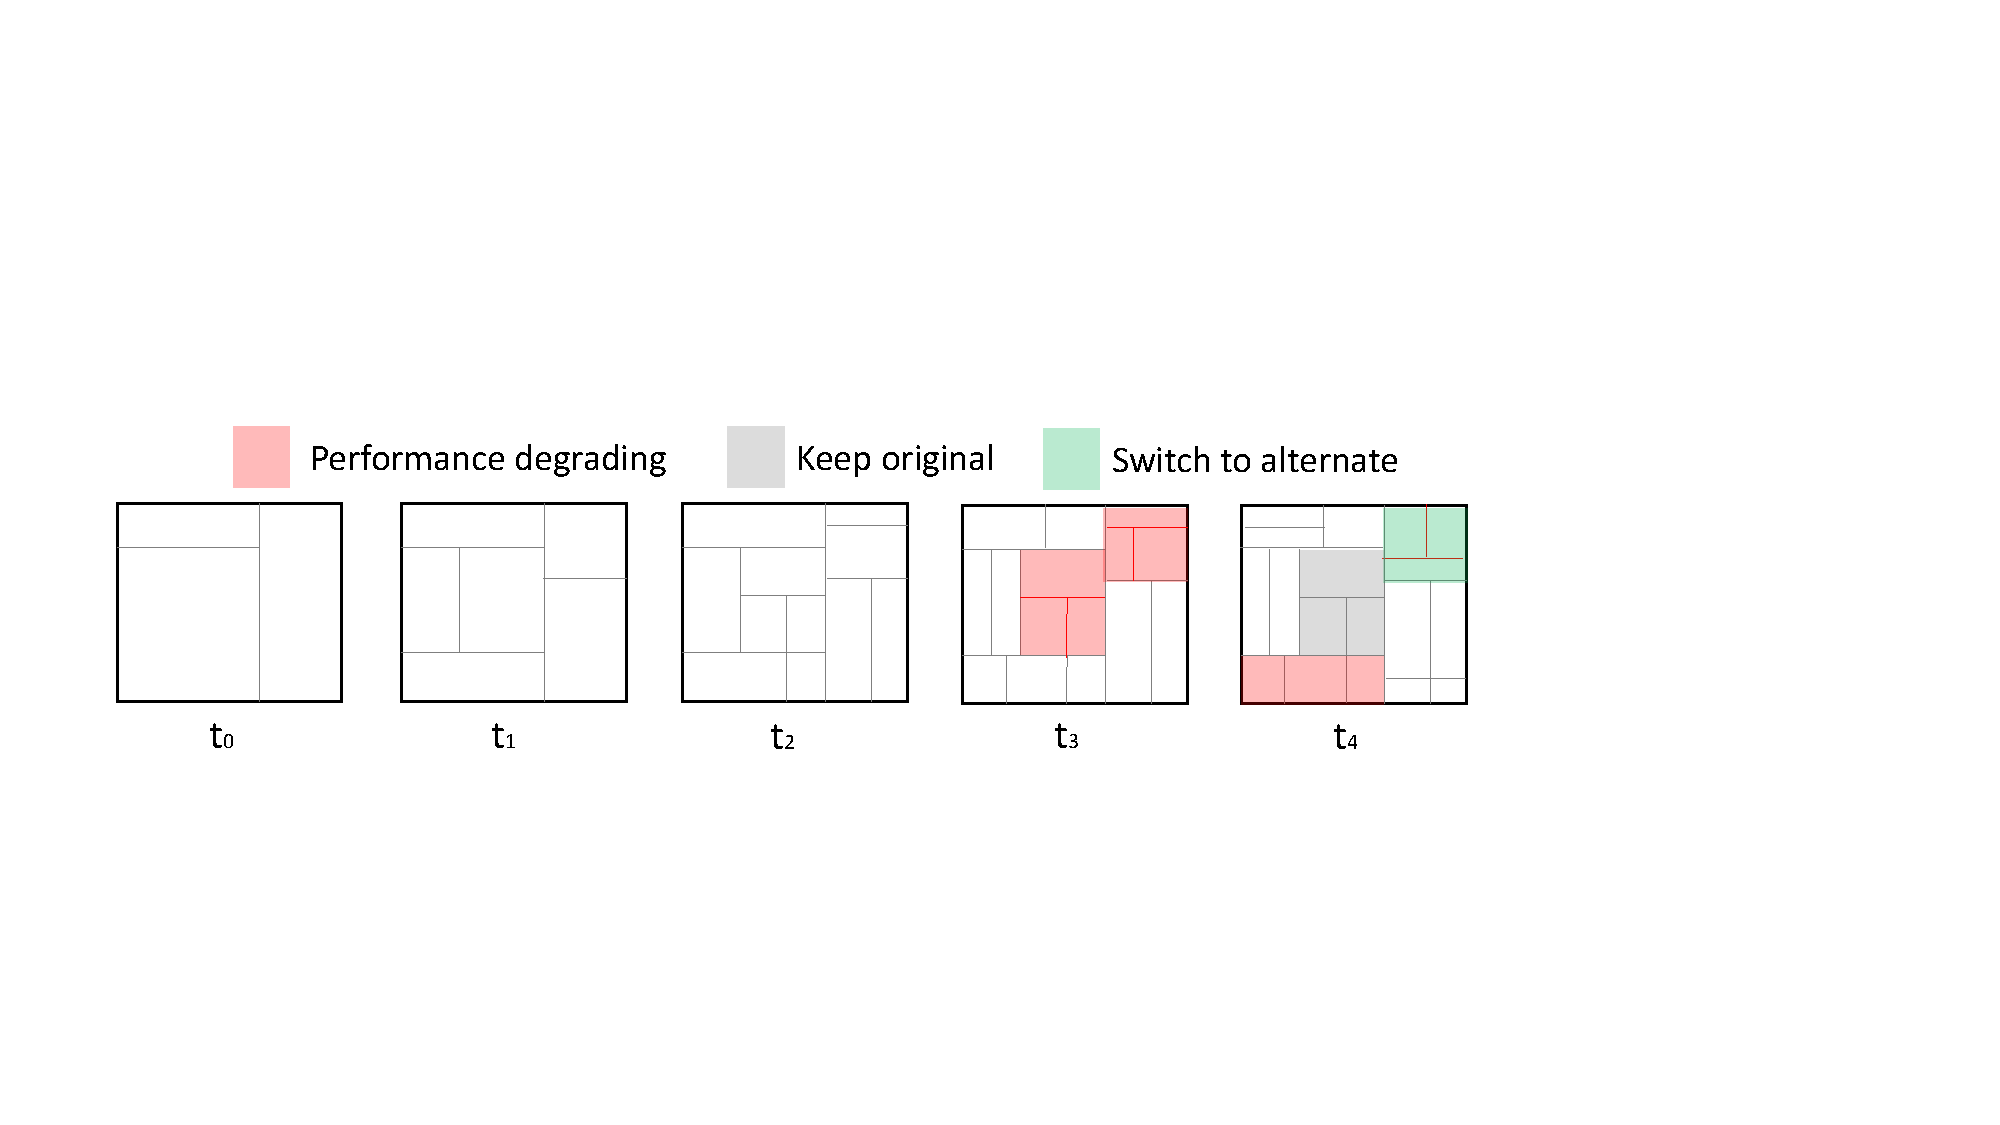
\includegraphics[width=14.0cm]{figs/prunedb.pdf}
        \caption{Decision boundaries after pruning using alternate branching}
        \label{fig:algo:prunedb}
    \end{center}
\end{figure}

\subsection{Combining the Ideas}
To approach our problem, we combine these ideas effectively. Our solution is entirely motivated by assumptions made in Hoeffding tree approaches, which is: to effectively decide on a splitting attribute in data streams with certain degree of accuracy, a small portion of the data is  sufficient; and the bound of accuracy can be estimated using Hoeffding bound. Based on this fundamental assumption, we combined the ideas of restricting and resetting Hoeffding tree based on a threshold size in terms of number of decision nodes, and the concept of maintaining alternate branches for nodes where performance are degrading using ADWIN method. Restricting the size of the tree can be used to control the amount of data the tree would be built upon. Applying ADWIN within the size restricted tree would ensure that the tree model is updated to the drifted concepts. 

As discussed earlier,  immediate reset of trees is not desirable where retaining  slower concepts is a concern. Thus, we developed a bagging scheme based on ASHT bagging to delay the reset of the trees upon reaching limit. With this scheme we stop the tree growth immediately as the size limitation is reached. We also start building a new tree with same size restriction. For the successive learning, both trees are learned with the exception that the old tree cannot grow. It may, however, switch to alternate branches. In cases, this might reduce the tree size and allow it to grow again. Switching to an alternate tree that would increase the tree size is not allowed. For the bagging, we thus maintain two sets of learners. One is same as the one from ASHT bagging. A fixed number of trees each with double the size of the previous one, first one being of size 2, typically. Other is initially empty with a fixed capacity. Once a tree in the first set reaches its limit it is moved to second set. The second set works as a fixed sized queue, as the newer trees are moved from the first set, older trees gets deleted. As the smaller trees reaches the size limit very fast, a threshold is set on the size of the trees that can be moved to the second set. The trees reaching their limit below this threshold are being reset immediately. In other words, we ``carry-over'' the larger the trees for a certain period of time even after reaching the max size limit. For the voting for a new instance, all classifier in both the sets contributes.

With this carrying-over concept, we essentially increase the weights of the decision rules in the larger trees, which directly influences the problem we are addressing. The larger trees contain decision rules for slower streams. By delaying the deletion of such trees, we create a buffer time for the new classifier to learn something from the newer data, while the older ones keep voting. The voting process remain more balanced between newer and older concepts during the transition period. Because in the transition time the new classifier with larger size limit, acts as a smaller classifier just because it has not seen enough data yet. This basically increases the voting bias towards newer concepts. With our  carry-over bagging, this becomes more balanced, as the larger trees would still keep voting for concepts present in older data. Algorithms devised based on the discussions above are explained in following sections.

\section{Size Restricted Hoeffding Tree (SRHT)}

\begin{algorithm}[htbp]
    \caption{SRHT: Size Restricted Hoeffding Tree}
    \label{alg:srht}
    \DontPrintSemicolon
    \SetKwInOut{Input}{Input} \SetKwInOut{Output}{Output} 
    
    \Input{$S$: Stream of examples \\
        $X$: Set of nominal attributes \\
        $Y$: Set of class labels $Y = \{y_1, y_2, \dots, y_k\}$ \\
        $G(.)$: Split evaluation function \\
        $N_{min}$: Minimum number of examples \\
        $\delta$: is one minus the desired probability \\
        $d$: Alternate tree switching bound \\
        $n_d$: Number of maximum decision nodes \\
        $\tau$: Constant to resolve ties
    } 
    \Output{$HT$: is a decision tree}
    
    \Begin{
        Let $HT \leftarrow$ Empty Leaf (Root) \\
        \ForEach{$example(x, y_k) \in S$} {
            Traverse the tree $HT$ from root till a leaf $l$ \\
            
            \eIf (\tcp*[f]{Missing class label}) {$y_k == ?$ } {
                Classify with majority class in the leaf $l$
            } {
                Update sufficient statistics \\
                \If{$ Number\;of\;examples\;in\;l > N_{min}$ }{
                    Compute $G_l(X_i)$ for all attributes \\
                    Let $X_a$ be the attribute with highest $G_l$ \\
                    Let $X_b$ be the attribute with second highest $G_l$ \\
                    Start maintaining ADWIN \\
                    
                    \uIf{error increased from previous step} {
                        Start maintaining alternate tree \\
                    }
                    \uElseIf{oldError - alternateError > $d$} {
                        \uIf{ADWIN window sufficiently big}{
                            Switch to alternate tree \\
                        }
                        \uElseIf{alternateError - oldError > $d$} {
                            Delete alternate tree \\
                        }
                    }
                    
                    Compute $\epsilon = \sqrt{\frac{R^2 \ln(2/\delta)}{2n}}$  \tcp*[f]{Hoeffding bound} \\
                    
                    \If{$G(X_a) - G(X_b) > \epsilon\; || \;\epsilon < \tau$} {
                        \If{decision node count < $n_d$} {
                            Replace $l$ with a splitting test based on attribute $X_a$ \\
                            Add a new empty leaf for each branch of the split \\
                        }
                    }
                }
            }
        }
    Return $HT$
    }
\end{algorithm}

Size Restricted Hoeffding Tree is an ADWIN variant of Adaptive Size Hoeffding Tree. It starts with an empty leaf or root. Every incoming instances is traversed to a leaf. The class label at the leaves are computed based on some base learners such as k-NN, naive Bayes, majority voting, etc. A grace period is imposed to reduce the number of unnecessary computations. Once a leaf gets predefined number of instances $N_{min}$, checking for branching is started. If a leaf is not pure, possibility for branching is checked. Hoeffding bound is applied here. The best two attributes  are chosen based on an information gain function. If the difference of gain between attributes is greater than the computed Hoeffding bound $\epsilon$ and total number of decision nodes is less a given threshold $n_d$, the leaf node is replaced with a decision node, and the instances weight are distributed among the new node's children. Additionally, ADWIN scheme is maintained at each decision nodes to check the error status. Whenever a decision node's performance starts falling, i.e. error increases, an alternate sub-tree for that node is created. Every instance reaching that node would be used to learn both the original and the alternate sub-trees. If the performance of any alternate subtree becomes better than the original sub-tree by a margin of $d$, the original sub-tree is replaced with the alternate one. Similarly, if the original sub-tree's performance improves again by a margin of $d$ the alternate trees are deleted. The use of margin $d$ ensures that, the classifier will not swing back and forth in case of similar and alternating concepts.

\section{Carry-over Bagging with SRHT}

SRHT is used in association with Carry-over Bagging (CoBag) ensemble approach. As SRHT is limited in terms of size, it will get outdated time to time, and would require to be replaced. This is done using carry-over bagging method.

\begin{algorithm}[htbp]
    \caption{CoBag: Carry-Over Bagging with SRHT}
    \label{alg:cobag}
    \DontPrintSemicolon
    \SetKwInOut{Input}{Input} \SetKwInOut{Output}{Output} 
    
    \Input{
        $H$: Set of base learners \\
        $n$: Ensemble size \\
        $m$: Additional ensemble size \\
        $b$: Tree size limit to use additional ensembles
    } 
    \Output{A SRHT ensemble}
    
    \Begin{
        Create $n$ SRHT $H_i$ \\
        Creating an empty ensemble with capacity $m$ \\
        \ForEach{$h \in H$} {
            Set $k$ according to $Poisson(1)$ \\
            \For{$i: 1-k$} {
                Learn $h$ with SRHT\\
                \uIf{$h.size > h.maxSize$ and $h.size < b$} {
                    Reset $h$ \\
                }
                \uElseIf {$h.size > h.maxSize$} {
                    Move $h$ to Alternate ensemble \\
                    Create new SRHT with size limit of $h.maxSize$ \\
                    
                    \If{Size of additional ensemble > m} {
                        Delete the oldest $h$ from additional ensemble \\
                    }
                }
            }
        }
        
    }

\end{algorithm}

Carry-over bagging methods is similar to the one used in ASHT bagging, which implements Oza online bagging approach. We use a similar approach with notable difference of using two different sets of classifiers for the ensemble. For the first set, a fixed number ($n$) of classifiers is initialized using different  size limits. Size of the smallest classifier is a user given value. Successive classifiers have a limit of twice the size of its immediate predecessor. As explained previously, this ensemble performs similarly to the one from ASHT bagging method. We introduced the second set with a capacity of $m$ classifiers to store the classifiers from first set when they reach their limit. Which classifiers are allowed to be stored in the second set is guarded by a threshold size, $b$. Hence, smaller classifiers being reset often do not affect the performance of overall process. When the second set becomes full, and there is new classifier to be added (that reached its limit), we deleted the oldest one from the set. For our experimentations, the size of the second set is kept equal to the size of first set, and the threshold is set to size of the median classifier. 


\section{Summary}
Before we start presenting the data set preparation and the experimental evaluation results, here is a brief summary of the investigated methods:

\textbf{Hoeffding Tree (HT)} With enough instances on an impure node checks for best two attributes. If their information gain difference satisfies Hoeffding bound, splits the node with best attribute.

\textbf{Adaptive Hoeffding Tree (AdaHT)} It uses ADWIN monitor to replace sub-trees if the performance starts degrading.

\textbf{Adaptive Size Hoeffding Tree (ASHT)} Reimplementation of Hoeffding tree with complete resetting or just root deleting capability.

\textbf{Bagging with Hoeffding Tree (BagHT)} Oza online bagging with Hoeffding tree. All the trees grows with time.

\textbf{Bagging with Adaptive Hoeffding Tree (BagHT)} Oza online bagging with adaptive Hoeffding tree. Trees grow indefinitely unless are replaced by ADWIN monitoring scheme.

\textbf{Bagging with Adaptive Size Hoeffding Tree (BagASHT)} Oza online bagging with ASHTs with different size limits.

\textbf{Bagging with Size Restricted Hoeffding Tree (BagSRHT/CoBagSRHT)} Carry-over bagging with SRHT with different size limits.

\textbf{Boosting with Hoeffding Tree (BoostHT)}  Oza online boosting with Hoeffding Tree.

\textbf{Boosting with Adaptive Hoeffding Tree (BoostAdaHT)} Oza online boosting with adaptive Hoeffding Tree.

\textbf{Boosting with ADWIN with Hoeffding Tree (BoostAdwin)} Oza online boosting where ensemble maintains ADWIN for classifiers (Hoeffding tree). Similar to BoostAdaHT.


\begin{table}[htbp]
    \caption{Comparison among various learners}
    \label{tab:treecomp}
    \vspace{-5mm}
    \begin{center}
    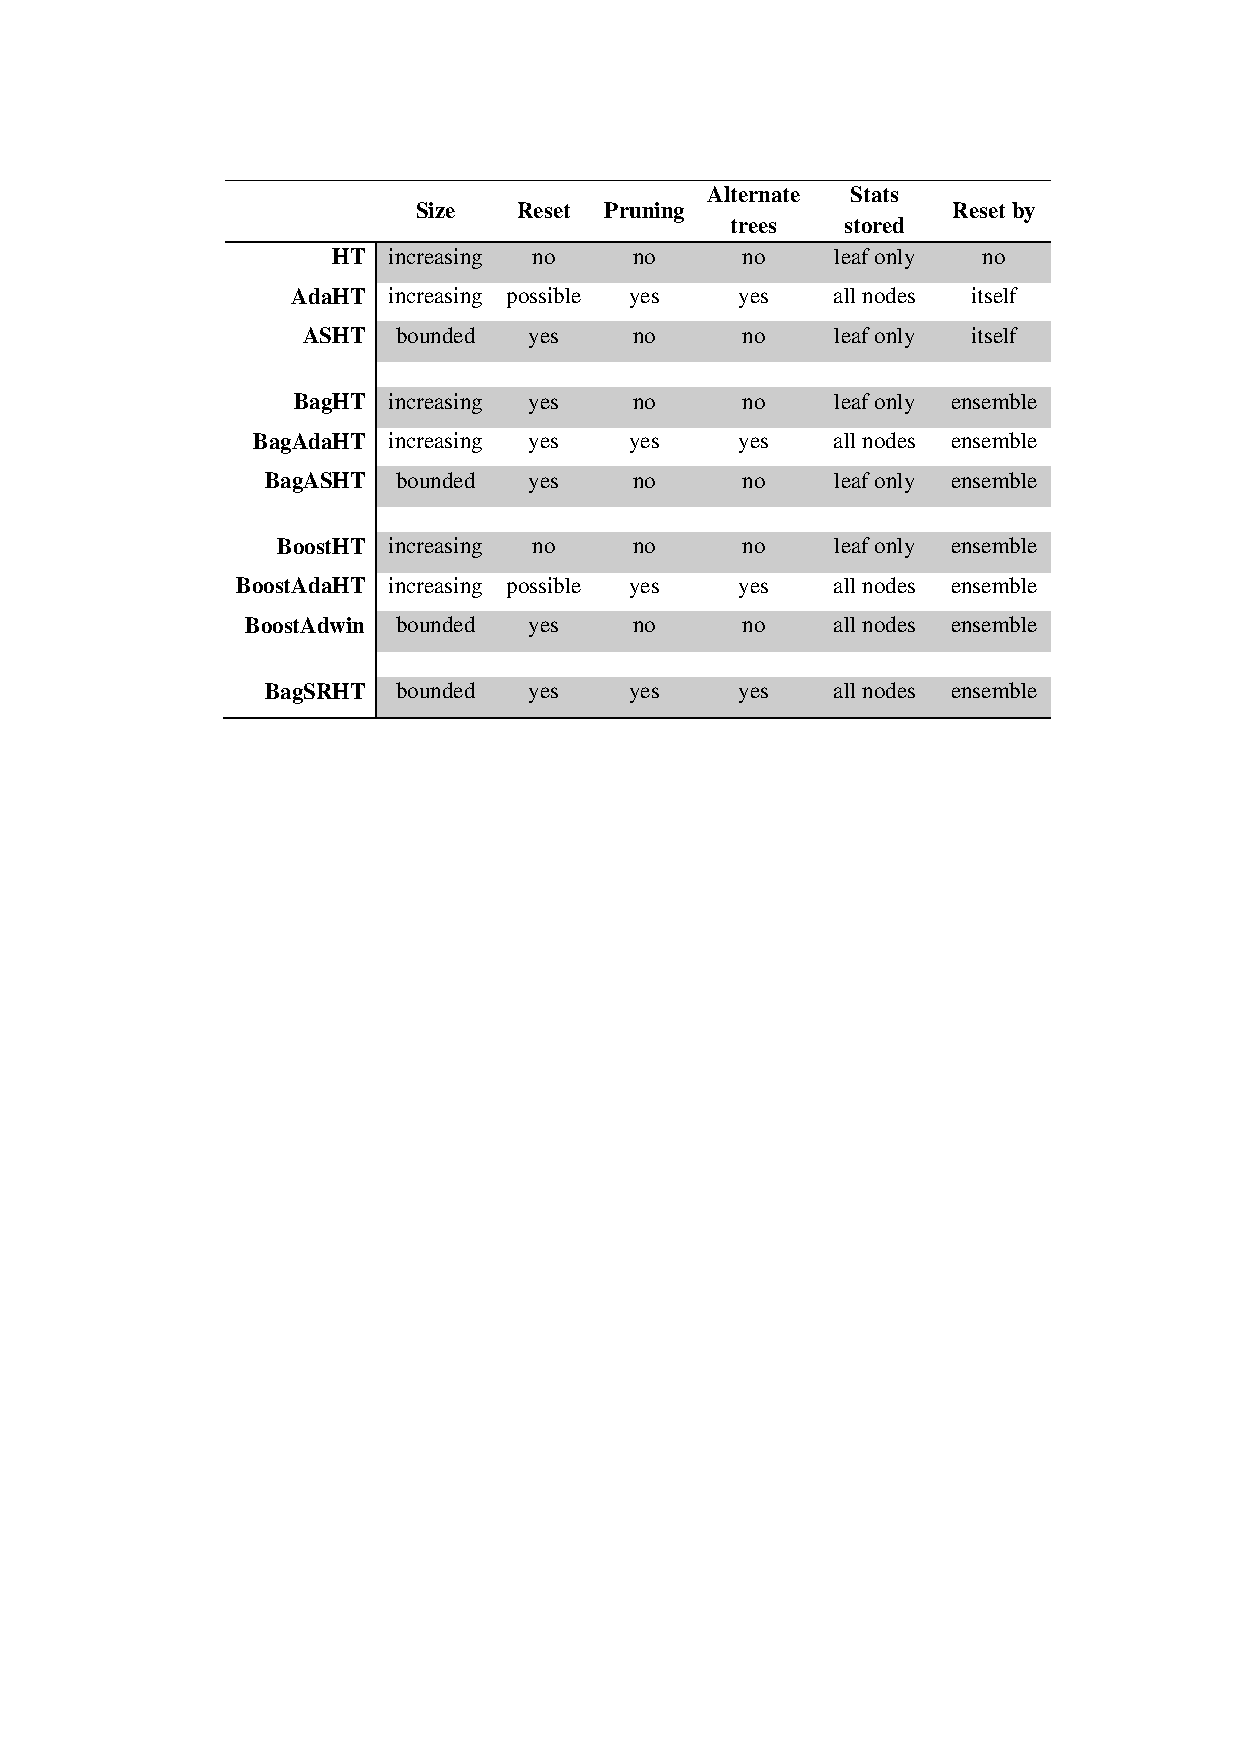
\includegraphics{figs/treescomp.pdf}
    \end{center}
\end{table}

